%************************************************
\section{Simulation Runtime} % (fold)
\label{sec:impl_simulation_runtime}
%************************************************
As depicted in Figure \ref{fig:final_architecture}, the Simulation Runtime component is responsible for loading up the 3D model of the target environment and initialize some of the components: the agent \ref{sec:impl_the_agent} and the monitoring service \ref{sec:impl_monitoring_service}. It also represents the entry point of the simulation. In Java terminology this means that this is the main class of the application.\\

Each simulation a system designer would set up, needs to follow the exact same series of tasks. Hence, this component represents an abstraction which must be extended by each particular simulation. Normally, the particular simulation should only provide the loaded scene and the abstraction takes care of the rest. We have implemented a few prototype simulations described in Section \ref{sec:impl_prototype_simulations}. These prototype simulations have been used during the evaluation process.\\

The diagram in Figure \ref{fig:impl_ego_app} illustrates the EgocentricApp abstract class and how it relates to some classes in the JME library. This abstraction provides the functionality needed for a concrete simulation. The diagram highlights only a few of its properties and methods.
\begin{figure}[H]
	\centering
	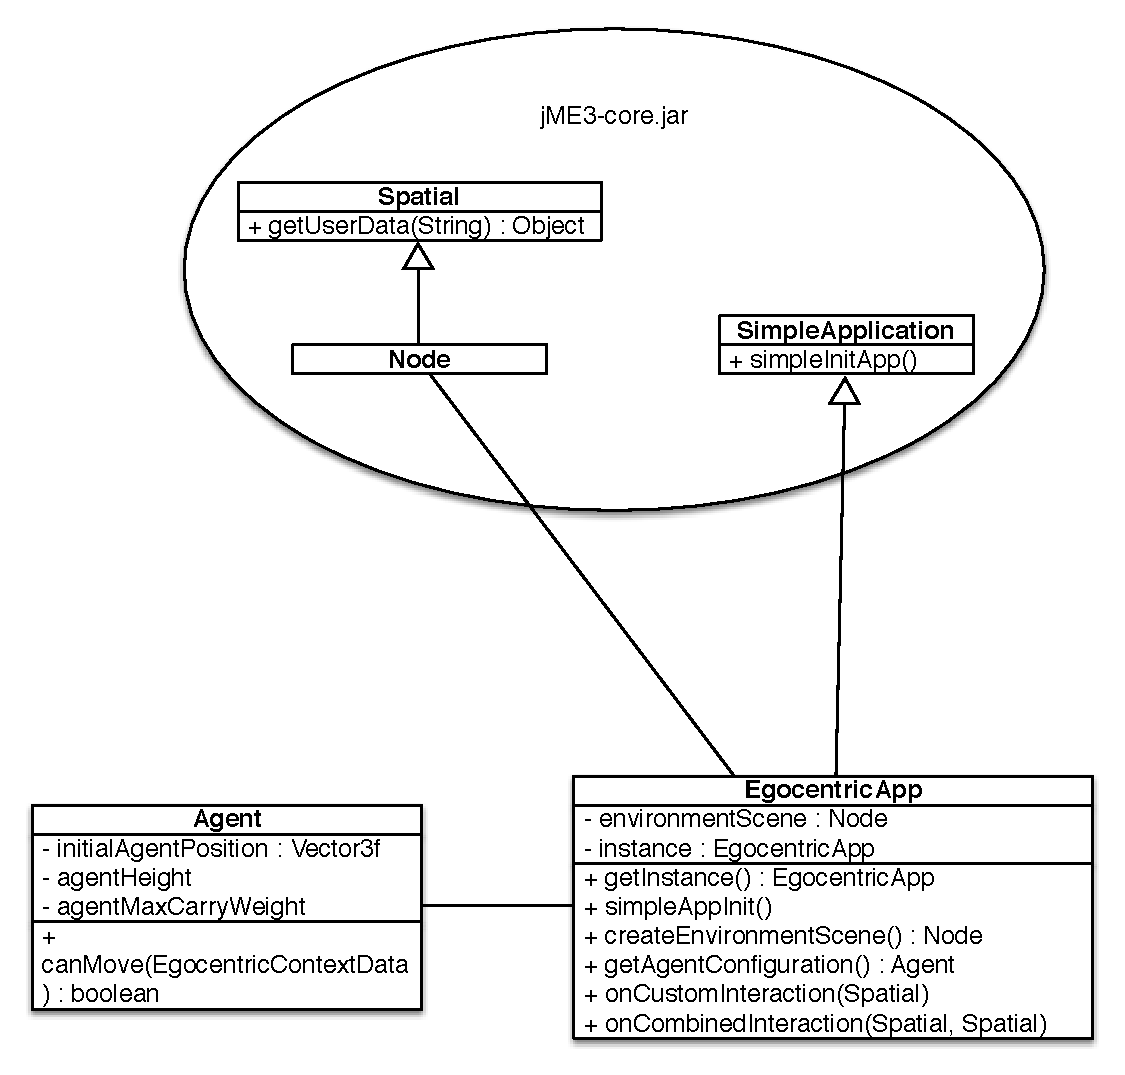
\includegraphics[width=\linewidth]{gfx/Chapter4/ego_app}
	\caption{EgocentricApp Class Diagram}
	\label{fig:impl_ego_app}
\end{figure}

The EgocentricApp subclasses SimpleApplication from the core JME library.  SimpleApplication  gives us access to standard game features, such as a scene graph (or the rootNode), an asset manager (to import textures, sounds, etc), a user interface (guiNode), input manager, audio manager, and many more. We have covered most of these concepts in Sections \ref{subsec:game_engine_architecture} and \ref{subsec:game_engine_concepts}. The components we have access through SimpleApplication are implementations of these generic concepts particular to JME. To star or stop the simulation, SimpleApplication provides the \emph{start()} and \emph{stop()} methods.\\

In the diagram, we have depicted the \emph{simpleInitApp()} method. This is called when the simulation is initialized. This is where EgocentricApp initializes of the simulation as follows:
\begin{enumerate}
	\item calls the \emph{createEnvironmentScene()}. This is an abstract method and must be implemented in all the subclasses. It must return an instance of a Node, meaning the subclass is not constrained to load the a certain type of 3D model. It can load any of the supported formats or even build the model pragmatically.
	\item it adds a collision control component to the environment scene. This will handle automatic collision detection with other collidable entities (i.e. the agent).
	\item add the environment scene to the guiNode. The environmentScene is just an in-memory data structure. To make it visible, it must be added to the rendered tree of nodes.
	\item start up the monitoring service
	\item create the first person agent using the Agent configuration data 
\end{enumerate}

Besides the createEnvironmentScene() method, all the other methods are implemented with a default behaviour. For example the getAgentConfiguration() method, provides various configuration parameters needed by the first person agent. More on the agent, in Section \ref{sec:impl_the_agent}.\\

The EgocentricApp provide two callback methods:
\begin{itemize}
	\item onCustomInteraction(Spatial) is called when the agent tries to interact with an object carrying Ego Metadata with a custom interactioType. The object is received as a parameter. This method can be overridden and a concrete simulation can implement various custom behaviours. For example, interacting with a door, should open it.
	\item onCombinedInteraction(Spatial, Spatial) is called when the agent tries to interact with an object while carrying a picked up object. For example, interacting with a notebook while carrying a pen, could pop up a window so the simulation user can easily input text.
\end{itemize}

Spatials are the elements of the 3D scene graph. As depicted in the class diagram they provide the \emph{getUserData(String)} method. With the help of this method we can retrieve the Ego Metadata using the EGOCENTRIC\_CONTEXT\_DATA flag. In the callback methods presented above, the received spatials will always carry Ego Metadata. Otherwise, the callback methods will not be called in the first place.\\

The simulation logic is spread among the components which we will present next. The EgocentricApp is mean to initialize these components and provide a generic entry point for the concrete simulations extending it. To provide easy access to various game assets and the callback methods for the rest of the components, EgocentricApp is implemented as Singleton \cite{gamma1994design}.\\

A few concrete simulation examples will be discussed in Section \ref{sec:impl_prototype_simulations}.
% section impl_simulation_runtime (end)